\section{Iteration 9: Decomposition of the Health Monitoring Unit}
\label{add:it9}

\subsection{Step 1: Identify candidate drivers}
\label{add:it9/drivers}

\npar Two quality attributes were assigned to the health monitoring unit:

\begin{itemize}
  	\item Av1': Measurement database failure. The failure is detected in less then five seconds.
  	\item Av2': Missing measurements. Failure of an internal component should be
  	detected within one minute.
\end{itemize}

\subsection{Step 2: Choose design concepts}
\label{add:it9/concepts}

\npar In this section there will be an overview of the chosen tactics and
patterns.

\subsubsection{Tactics}
\label{add:it9/tactics}

\npar Since only the detection part of the availability attributes was assigned
to the health monitoring unit, the tactics used in this iteration will be based
upon that assumption. In section \ref{add:it1} we discussed the best detection
tactic and this resulted in the usage of a heartbeat. The usage of heartbeat
will be the (only) tactic in this iteration.

\subsubsection{Design Patterns}
\label{add:it9/patterns}

\npar There was no design pattern found to support the notification
functionality in combination with the heartbeat tactic.

\subsection{Step 3: Instantiate architectural elements and allocate responsibilities}
\label{add:it9/elements}

\begin{figure}[H]
	\begin{centering}
		% TODO Figure
		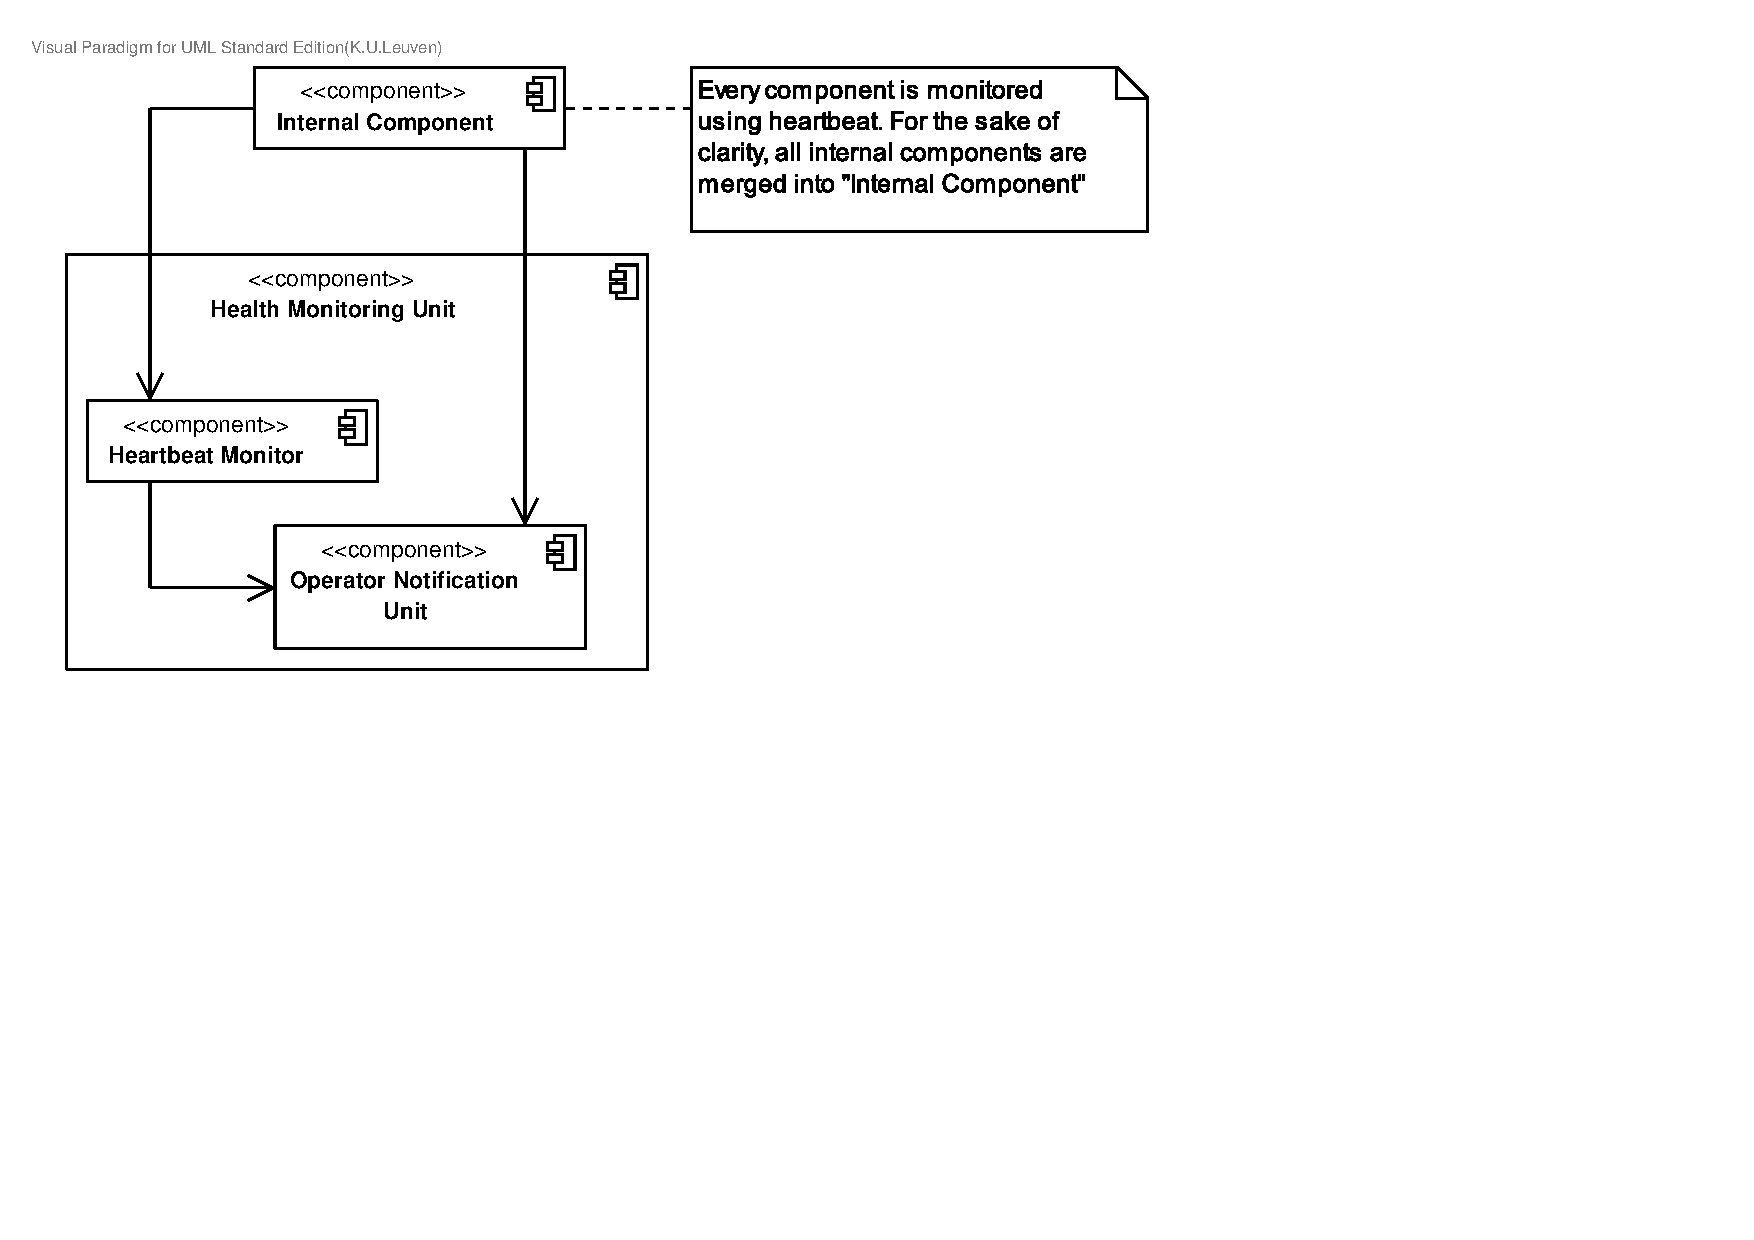
\includegraphics[width=\textwidth]{figs/add-it9-elements.pdf}
		\caption{Overview of the instantiated child elements in the Health Monitoring
		Unit.}
		\label{fig:it9/elements}
	\end{centering}
\end{figure}

\npar The design is relatively simple. There are only two components, they are
together with all their associations depicted in figure \ref{fig:it9/elements}.

\subsubsection{OperatorNotificationUnit}

\npar This unit is purely responsible for the notification of ReMeS operators. A
notification request can enter this unit either from the heartbeat monitor or
from an external component.

\subsubsection{HeartbeatMonitor}

\npar The HeartbeatMonitor is a registering point for other components to
confirm that they are still up and running. When a component does not give a
heartbeat signal, it is assumed that that component is crashed and approriate
action is undertaken (i.e. a ReMeS operator is notified). Off course it is
always possible that the monitor itself fails. Therefore this component is in
fact a cluster of monitors where each monitor monitors every other monitor.

\subsection{Step 4: Define interfaces for instantiated elements}
\label{add:it9/interfaces}

\npar In this section each interface is explained in terms of the components
which use and/or offer it together with information about what is exchanged. For
detailed information with reference to the specific methods the interfaces
implement, we refer to the interface catalog, see appendix
\ref{chap:interface-catalog}.

\subsubsection{HealthMonitorAPI}

\npar The \interface{HealthMonitorAPI} was already discussed in section
\ref{add:it1/interfaces}.

\subsubsection{OperatorNotificationAPI}

\npar This interface lies in between the OperatorNotificationUnit and components
who need to be able to notify a ReMeS operator. 

\begin{figure}[H]
	\begin{centering}
		% TODO Figure
		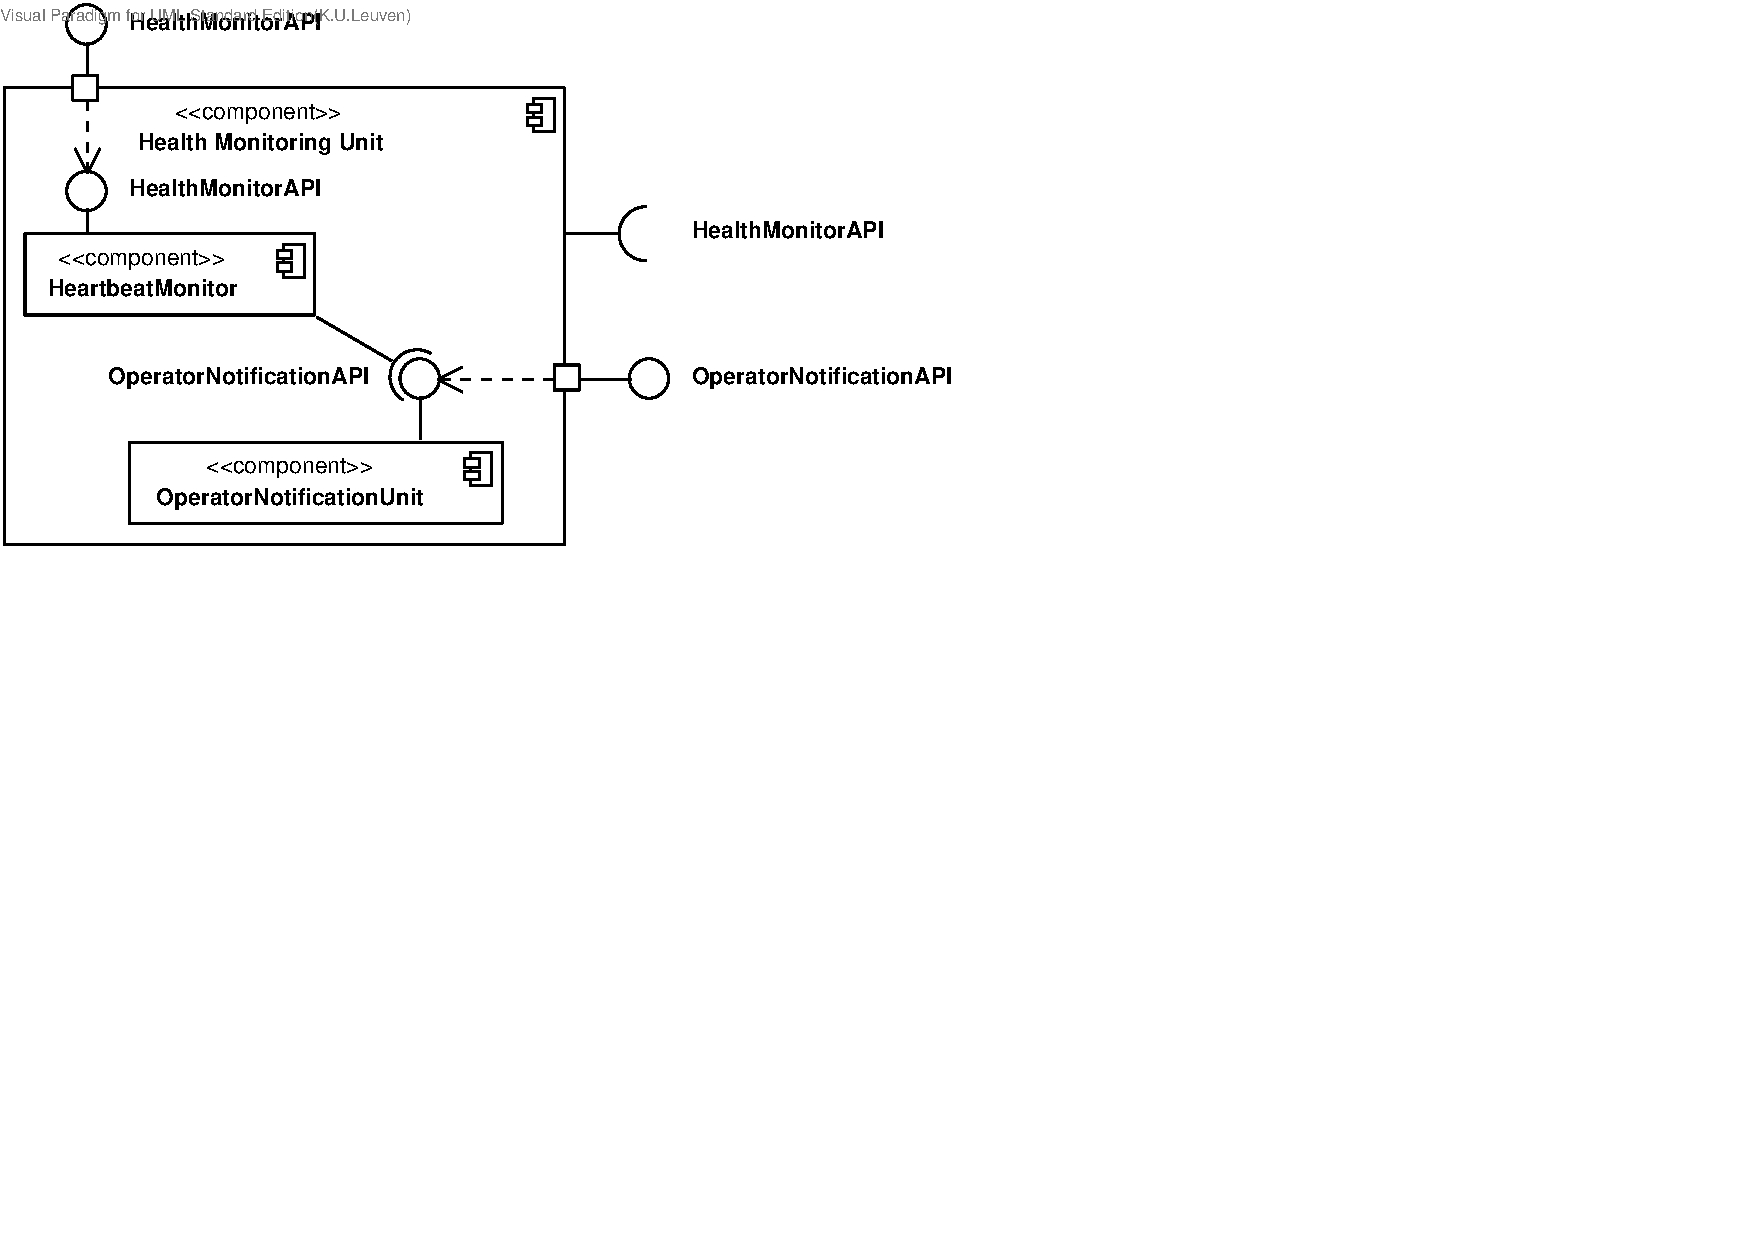
\includegraphics[width=\textwidth]{figs/add-it9-interfaces.pdf}
		\caption{Overview of the interfaces and components in the Health Monitoring
		Unit.}
		\label{fig:it9/interfaces}
	\end{centering}
\end{figure}

\subsection{Step 5: Verify and refine}
\label{add:it9/verification}

\npar The assigned parts of Av1' and Av2' were resolved in this iteration
through the use of the Heartbeat Monitor and the Operator Notification Unit.
